\documentclass{ximera}

%\usepackage{todonotes}

\newcommand{\todo}{}

\usepackage{esint} % for \oiint
\ifxake%%https://math.meta.stackexchange.com/questions/9973/how-do-you-render-a-closed-surface-double-integral
\renewcommand{\oiint}{{\large\bigcirc}\kern-1.56em\iint}
\fi


\graphicspath{
  {./}
  {ximeraTutorial/}
  {basicPhilosophy/}
  {functionsOfSeveralVariables/}
  {normalVectors/}
  {lagrangeMultipliers/}
  {vectorFields/}
  {greensTheorem/}
  {shapeOfThingsToCome/}
  {dotProducts/}
  {partialDerivativesAndTheGradientVector/}
  {../productAndQuotientRules/exercises/}
  {../normalVectors/exercisesParametricPlots/}
  {../continuityOfFunctionsOfSeveralVariables/exercises/}
  {../partialDerivativesAndTheGradientVector/exercises/}
  {../directionalDerivativeAndChainRule/exercises/}
  {../commonCoordinates/exercisesCylindricalCoordinates/}
  {../commonCoordinates/exercisesSphericalCoordinates/}
  {../greensTheorem/exercisesCurlAndLineIntegrals/}
  {../greensTheorem/exercisesDivergenceAndLineIntegrals/}
  {../shapeOfThingsToCome/exercisesDivergenceTheorem/}
  {../greensTheorem/}
  {../shapeOfThingsToCome/}
  {../separableDifferentialEquations/exercises/}
  {vectorFields/}
}

\newcommand{\mooculus}{\textsf{\textbf{MOOC}\textnormal{\textsf{ULUS}}}}

\usepackage{tkz-euclide}
\usepackage{tikz}
\usepackage{tikz-cd}
\usetikzlibrary{arrows}
\tikzset{>=stealth,commutative diagrams/.cd,
  arrow style=tikz,diagrams={>=stealth}} %% cool arrow head
\tikzset{shorten <>/.style={ shorten >=#1, shorten <=#1 } } %% allows shorter vectors

\usetikzlibrary{backgrounds} %% for boxes around graphs
\usetikzlibrary{shapes,positioning}  %% Clouds and stars
\usetikzlibrary{matrix} %% for matrix
\usepgfplotslibrary{polar} %% for polar plots
\usepgfplotslibrary{fillbetween} %% to shade area between curves in TikZ
%\usetkzobj{all}
\usepackage[makeroom]{cancel} %% for strike outs
%\usepackage{mathtools} %% for pretty underbrace % Breaks Ximera
%\usepackage{multicol}
\usepackage{pgffor} %% required for integral for loops



%% http://tex.stackexchange.com/questions/66490/drawing-a-tikz-arc-specifying-the-center
%% Draws beach ball
\tikzset{pics/carc/.style args={#1:#2:#3}{code={\draw[pic actions] (#1:#3) arc(#1:#2:#3);}}}



\usepackage{array}
\setlength{\extrarowheight}{+.1cm}
\newdimen\digitwidth
\settowidth\digitwidth{9}
\def\divrule#1#2{
\noalign{\moveright#1\digitwidth
\vbox{\hrule width#2\digitwidth}}}




% \newcommand{\RR}{\mathbb R}
% \newcommand{\R}{\mathbb R}
% \newcommand{\N}{\mathbb N}
% \newcommand{\Z}{\mathbb Z}

\newcommand{\sagemath}{\textsf{SageMath}}


%\renewcommand{\d}{\,d\!}
%\renewcommand{\d}{\mathop{}\!d}
%\newcommand{\dd}[2][]{\frac{\d #1}{\d #2}}
%\newcommand{\pp}[2][]{\frac{\partial #1}{\partial #2}}
% \renewcommand{\l}{\ell}
%\newcommand{\ddx}{\frac{d}{\d x}}

% \newcommand{\zeroOverZero}{\ensuremath{\boldsymbol{\tfrac{0}{0}}}}
%\newcommand{\inftyOverInfty}{\ensuremath{\boldsymbol{\tfrac{\infty}{\infty}}}}
%\newcommand{\zeroOverInfty}{\ensuremath{\boldsymbol{\tfrac{0}{\infty}}}}
%\newcommand{\zeroTimesInfty}{\ensuremath{\small\boldsymbol{0\cdot \infty}}}
%\newcommand{\inftyMinusInfty}{\ensuremath{\small\boldsymbol{\infty - \infty}}}
%\newcommand{\oneToInfty}{\ensuremath{\boldsymbol{1^\infty}}}
%\newcommand{\zeroToZero}{\ensuremath{\boldsymbol{0^0}}}
%\newcommand{\inftyToZero}{\ensuremath{\boldsymbol{\infty^0}}}



% \newcommand{\numOverZero}{\ensuremath{\boldsymbol{\tfrac{\#}{0}}}}
% \newcommand{\dfn}{\textbf}
% \newcommand{\unit}{\,\mathrm}
% \newcommand{\unit}{\mathop{}\!\mathrm}
% \newcommand{\eval}[1]{\bigg[ #1 \bigg]}
% \newcommand{\seq}[1]{\left( #1 \right)}
% \renewcommand{\epsilon}{\varepsilon}
% \renewcommand{\phi}{\varphi}


% \renewcommand{\iff}{\Leftrightarrow}

% \DeclareMathOperator{\arccot}{arccot}
% \DeclareMathOperator{\arcsec}{arcsec}
% \DeclareMathOperator{\arccsc}{arccsc}
% \DeclareMathOperator{\si}{Si}
% \DeclareMathOperator{\scal}{scal}
% \DeclareMathOperator{\sign}{sign}


%% \newcommand{\tightoverset}[2]{% for arrow vec
%%   \mathop{#2}\limits^{\vbox to -.5ex{\kern-0.75ex\hbox{$#1$}\vss}}}
% \newcommand{\arrowvec}[1]{{\overset{\rightharpoonup}{#1}}}
% \renewcommand{\vec}[1]{\arrowvec{\mathbf{#1}}}
% \renewcommand{\vec}[1]{{\overset{\boldsymbol{\rightharpoonup}}{\mathbf{#1}}}}

% \newcommand{\point}[1]{\left(#1\right)} %this allows \vector{ to be changed to \vector{ with a quick find and replace
% \newcommand{\pt}[1]{\mathbf{#1}} %this allows \vec{ to be changed to \vec{ with a quick find and replace
% \newcommand{\Lim}[2]{\lim_{\point{#1} \to \point{#2}}} %Bart, I changed this to point since I want to use it.  It runs through both of the exercise and exerciseE files in limits section, which is why it was in each document to start with.

% \DeclareMathOperator{\proj}{\mathbf{proj}}
% \newcommand{\veci}{{\boldsymbol{\hat{\imath}}}}
% \newcommand{\vecj}{{\boldsymbol{\hat{\jmath}}}}
% \newcommand{\veck}{{\boldsymbol{\hat{k}}}}
% \newcommand{\vecl}{\vec{\boldsymbol{\l}}}
% \newcommand{\uvec}[1]{\mathbf{\hat{#1}}}
% \newcommand{\utan}{\mathbf{\hat{t}}}
% \newcommand{\unormal}{\mathbf{\hat{n}}}
% \newcommand{\ubinormal}{\mathbf{\hat{b}}}

% \newcommand{\dotp}{\bullet}
% \newcommand{\cross}{\boldsymbol\times}
% \newcommand{\grad}{\boldsymbol\nabla}
% \newcommand{\divergence}{\grad\dotp}
% \newcommand{\curl}{\grad\cross}
%\DeclareMathOperator{\divergence}{divergence}
%\DeclareMathOperator{\curl}[1]{\grad\cross #1}
% \newcommand{\lto}{\mathop{\longrightarrow\,}\limits}

% \renewcommand{\bar}{\overline}

\colorlet{textColor}{black}
\colorlet{background}{white}
\colorlet{penColor}{blue!50!black} % Color of a curve in a plot
\colorlet{penColor2}{red!50!black}% Color of a curve in a plot
\colorlet{penColor3}{red!50!blue} % Color of a curve in a plot
\colorlet{penColor4}{green!50!black} % Color of a curve in a plot
\colorlet{penColor5}{orange!80!black} % Color of a curve in a plot
\colorlet{penColor6}{yellow!70!black} % Color of a curve in a plot
\colorlet{fill1}{penColor!20} % Color of fill in a plot
\colorlet{fill2}{penColor2!20} % Color of fill in a plot
\colorlet{fillp}{fill1} % Color of positive area
\colorlet{filln}{penColor2!20} % Color of negative area
\colorlet{fill3}{penColor3!20} % Fill
\colorlet{fill4}{penColor4!20} % Fill
\colorlet{fill5}{penColor5!20} % Fill
\colorlet{gridColor}{gray!50} % Color of grid in a plot

\newcommand{\surfaceColor}{violet}
\newcommand{\surfaceColorTwo}{redyellow}
\newcommand{\sliceColor}{greenyellow}




\pgfmathdeclarefunction{gauss}{2}{% gives gaussian
  \pgfmathparse{1/(#2*sqrt(2*pi))*exp(-((x-#1)^2)/(2*#2^2))}%
}


%%%%%%%%%%%%%
%% Vectors
%%%%%%%%%%%%%

%% Simple horiz vectors
\renewcommand{\vector}[1]{\left\langle #1\right\rangle}


%% %% Complex Horiz Vectors with angle brackets
%% \makeatletter
%% \renewcommand{\vector}[2][ , ]{\left\langle%
%%   \def\nextitem{\def\nextitem{#1}}%
%%   \@for \el:=#2\do{\nextitem\el}\right\rangle%
%% }
%% \makeatother

%% %% Vertical Vectors
%% \def\vector#1{\begin{bmatrix}\vecListA#1,,\end{bmatrix}}
%% \def\vecListA#1,{\if,#1,\else #1\cr \expandafter \vecListA \fi}

%%%%%%%%%%%%%
%% End of vectors
%%%%%%%%%%%%%

%\newcommand{\fullwidth}{}
%\newcommand{\normalwidth}{}



%% makes a snazzy t-chart for evaluating functions
%\newenvironment{tchart}{\rowcolors{2}{}{background!90!textColor}\array}{\endarray}

%%This is to help with formatting on future title pages.
\newenvironment{sectionOutcomes}{}{}



%% Flowchart stuff
%\tikzstyle{startstop} = [rectangle, rounded corners, minimum width=3cm, minimum height=1cm,text centered, draw=black]
%\tikzstyle{question} = [rectangle, minimum width=3cm, minimum height=1cm, text centered, draw=black]
%\tikzstyle{decision} = [trapezium, trapezium left angle=70, trapezium right angle=110, minimum width=3cm, minimum height=1cm, text centered, draw=black]
%\tikzstyle{question} = [rectangle, rounded corners, minimum width=3cm, minimum height=1cm,text centered, draw=black]
%\tikzstyle{process} = [rectangle, minimum width=3cm, minimum height=1cm, text centered, draw=black]
%\tikzstyle{decision} = [trapezium, trapezium left angle=70, trapezium right angle=110, minimum width=3cm, minimum height=1cm, text centered, draw=black]


\title{Transform Shape}

\begin{document}

\begin{abstract}
graphs
\end{abstract}
\maketitle



We now have four graphical transformations:


\begin{itemize}
\item horizontal shift
\item horizontal stretch or compression
\item vertical shift
\item vertical stretch or compression
\end{itemize}






$\blacktriangleright$  \textbf{\textcolor{purple!85!blue}{Horizontal - (inside)}}  \\


The horizontal transformations are controlled by multiplication and addition inside the domain parentheses in the function's formula.

\[      f(x) \longrightarrow   f(A \cdot x + B)  \]

Multiplication on the domain variable results in horizontal stretching or compression. \\
Addition results in horizontal shifting. \\





$\blacktriangleright$   \textbf{\textcolor{purple!85!blue}{Vertical - (outside)}}  \\



The vertical transformations are controlled by multiplication and addition outside on the function's formula.

\[      f(x) \longrightarrow   C \cdot f(x) + D \]

Multiplication on the function results in vertical stretching or compression. \\
Addition results in vertical shifting. \\





The visual or graphical horizontal effects of arithmetic performed on the domain are reverse of the arithmetic, because  there is a new function with its own new variable and the arithmetic shown to us is performed on this new variable.  The graphical transformations follow the arithmetic on the old/original variable.


From the original function, $f(x)$, we define a new function, $g(k)$.
\[
g(k) = f(A \cdot k + B)
\]


\[
x = A \cdot k + B
\]



To see what happens to the original variable, $x$, we need to solve for the new variable, which reverses all of the arithmetic. \\


\[
\frac{x - B}{A} = k
\]



The new variable, $k$, is obtained from the old variable, $x$, by subtracting $B$ and then dividing by $A$. \\


The visual or graphical vertical effects of arithmetic performed on the function are the same as the arithmetic, because they are applied directly to the original range variable, the function value - the dependent variable.










\begin{example} A Little Bit of Everything




Graph of $y = G(h)$, the original (basic) function.

\begin{image}
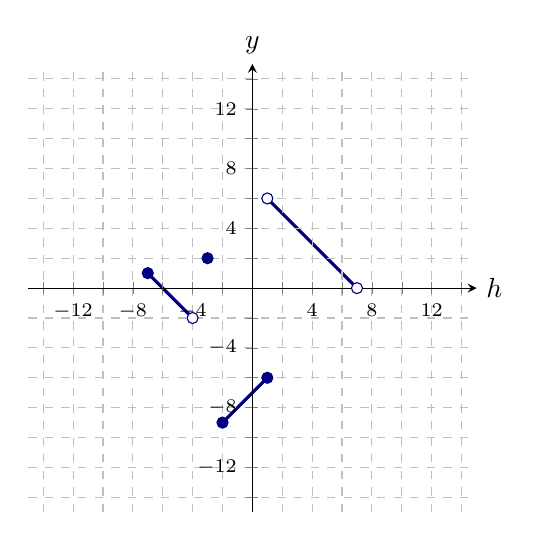
\begin{tikzpicture}
	\begin{axis}[
            domain=-15:15, ymax=15, xmax=15, ymin=-15, xmin=-15, unit vector ratio*=1 1 1,
            grid = both, grid style={dashed},
            ytick={-14,-12,-10,-8,-6,-4,-2,2,4,6,8,10,12,14}, xtick={-14,-12,-10,-8,-6,-4,-2,2,4,6,8,10,12,14},
            yticklabels={ , $-12$, , $-8$, ,$-4$, , ,$4$, ,$8$, ,$12$}, xticklabels={ , $-12$, , $-8$, ,$-4$, , ,$4$, ,$8$, ,$12$},
            ticklabel style={font=\scriptsize},
            axis lines =center, xlabel=$h$, ylabel=$y$,
            every axis y label/.style={at=(current axis.above origin),anchor=south},
            every axis x label/.style={at=(current axis.right of origin),anchor=west},
            axis on top
          ]
          
	\addplot [draw=penColor,very thick,smooth,domain=(-7:-4)] {-x-6};
	\addplot [draw=penColor,very thick,smooth,domain=(-2:1)] {x-7};
	\addplot [draw=penColor,very thick,smooth,domain=(1:7)] {-x+7};

	\addplot[color=penColor,only marks,mark=*] coordinates{(-3,2)}; 
	
	\addplot[color=penColor,only marks,mark=*] coordinates{(-7,1)}; 
	\addplot[color=penColor,fill=white,only marks,mark=*] coordinates{(-4,-2)}; 
	\addplot[color=penColor,only marks,mark=*] coordinates{(-2,-9)}; 
	\addplot[color=penColor,only marks,mark=*] coordinates{(1,-6)}; 
	\addplot[color=penColor,fill=white,only marks,mark=*] coordinates{(1,6)}; 
	\addplot[color=penColor,fill=white,only marks,mark=*] coordinates{(7,0)}; 


    \end{axis}
\end{tikzpicture}
\end{image}








\begin{itemize}

\item The domain of $G$ is $[-7,-4) \cup \{-3\} \cup [-2,7)$.
\item $G$ has no global maximum
\item $G$ has a global (and local) minimum of $\answer{-9}$, which occurs at $\answer{-2}$. 
\item $G$ has a local maximum of $1$, which occurs at $\answer{-7}$.
\item $G$ has both a local minimum and local maximum of $2$, which occurs at $-3$.
\end{itemize}





$\blacktriangleright$ Now to define a new function based on $G$.






Define  $T(p) = -2G\left( \frac{1}{2} p - 4 \right) + 1$.


How do we construct the graph of $z = T(p) = -2G\left(\frac{1}{2} p - 4\right) + 1$?

First, let's map over all of the endpoints in the graph of $y = G(h)$.

Remember: If  $h = \frac{1}{2} p - 4$, then $p = \answer{2(h+4)}$.

\begin{itemize}
 \item \textbf{Domain:}  $2 (h+4)$ 
    \begin{itemize}
      \item (1) add $4$
      \item (2) multiply by $2$
    \end{itemize}

 \item \textbf{Range:}  $-2 G + 1$ 
    \begin{itemize}
      \item (1) multiply by $-2$
      \item (2) add $1$
    \end{itemize}
\end{itemize}


First, we'll transform the domain coordinate, which is the left coordinate.  Then we'll transform the range coordinate, which is the right coordinate.

\[
\begin{array}{c|l|l|l|l|l}
        &         &  \text{domain}  &  \text{domain}    &  \text{range}   & \text{range}         \\
\text{Point}    &  \text{Original}  &  +4           &  \times2   &  \times(-2)  & + 1          \\
\hline
A   &   (-7, 1)          &  (-3, 1)      &  (-6, 1)     &  (-6, -2)    &  (-6,-1)     \\
B   &   (-4, -2)         &  (0, -2)      &  (0, -2)     &  (0,4)      &  (0,5)       \\
C   &   (-3,2)           &  (1,2)        &  (2,2)       &  (2,-4)     &  (2,-3)     \\
D   &   (-2,-9)          &  (2, -9)      &  (4,-9)      &  (4, 18)    &  (4,19)      \\
E   &   (1,-6)           &  (5,-6)       &  (10,-6)     &  (10,12)    &  (10,13)     \\
F   &   (1,6)            &  (5, 6)       &  (10,6)      &  (10,-12)   &  (10,-11)   \\
H   &   (7,0)            &  (11,0)       &  (22,0)      &  (22,0)     &  (22,1)
\end{array}
\]




Now, we'll graphically map the important points from $y=G(h)$ to $t = T(p)$:
















\begin{image}
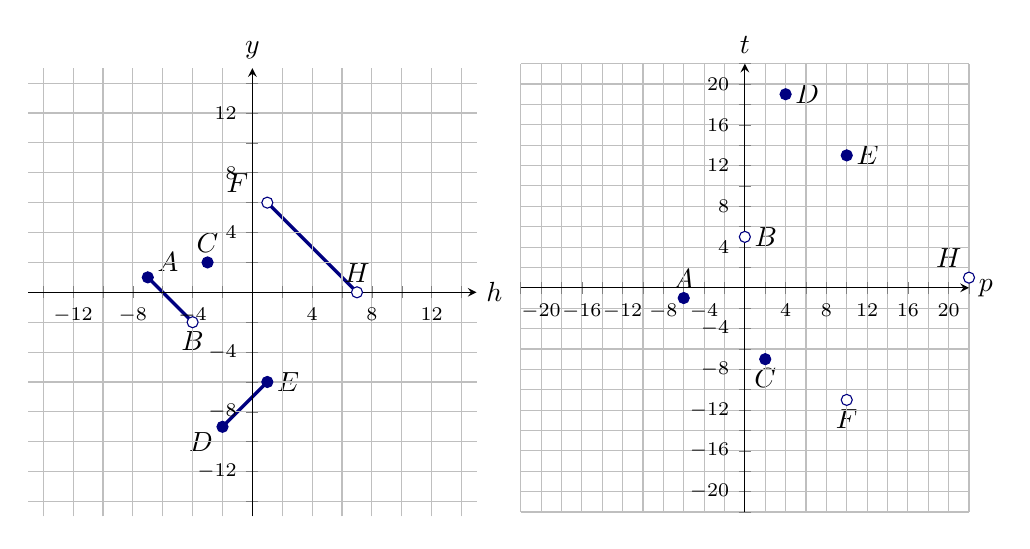
\begin{tikzpicture}
  \begin{axis}[name = leftgraph,
            domain=-15:15, ymax=15, xmax=15, ymin=-15, xmin=-15, unit vector ratio*=1 1 1,
            grid = both, 
            ytick={-14,-12,-10,-8,-6,-4,-2,2,4,6,8,10,12,14}, xtick={-14,-12,-10,-8,-6,-4,-2,2,4,6,8,10,12,14},
            yticklabels={ , $-12$, , $-8$, ,$-4$, , ,$4$, ,$8$, ,$12$}, xticklabels={ , $-12$, , $-8$, ,$-4$, , ,$4$, ,$8$, ,$12$},
            ticklabel style={font=\scriptsize},
            axis lines =center, xlabel=$h$, ylabel=$y$,
            every axis y label/.style={at=(current axis.above origin),anchor=south},
            every axis x label/.style={at=(current axis.right of origin),anchor=west},
            axis on top
          ]
          
        \addplot [draw=penColor,very thick,smooth,domain=(-7:-4)] {-x-6};
        \addplot [draw=penColor,very thick,smooth,domain=(-2:1)] {x-7};
        \addplot [draw=penColor,very thick,smooth,domain=(1:7)] {-x+7};

        \addplot[color=penColor,only marks,mark=*] coordinates{(-3,2)}; 
  
        \addplot[color=penColor,only marks,mark=*] coordinates{(-7,1)}; 
        \addplot[color=penColor,fill=white,only marks,mark=*] coordinates{(-4,-2)}; 
        \addplot[color=penColor,only marks,mark=*] coordinates{(-2,-9)}; 
        \addplot[color=penColor,only marks,mark=*] coordinates{(1,-6)}; 
        \addplot[color=penColor,fill=white,only marks,mark=*] coordinates{(1,6)}; 
        \addplot[color=penColor,fill=white,only marks,mark=*] coordinates{(7,0)}; 



        \node at (axis cs:-7,2) [anchor=west] {$A$};  
        \node at (axis cs:-4,-2) [anchor=north] {$B$};  
        \node at (axis cs:-3,2) [anchor=south] {$C$};  
        \node at (axis cs:-2,-10) [anchor=east] {$D$};
        \node at (axis cs:1,-6) [anchor=west] {$E$};
        \node at (axis cs:-1,6) [anchor=south] {$F$};
        \node at (axis cs:7,0) [anchor=south] {$H$};

    \end{axis}
  \begin{axis}[at={(leftgraph.outer east)},anchor=outer west,
            domain=-22:22, ymax=22, xmax=22, ymin=-22, xmin=-22, unit vector ratio*=1 1 1,
            grid = both, 
            ytick={-22,-20,-18,-16,-14,-12,-10,-8,-6,-4,-2,2,4,6,8,10,12,14,16,18,20,22}, xtick={-22,-20,-18,-16,-14,-12,-10,-8,-6,-4,-2,2,4,6,8,10,12,14,16,18,20,22},
            yticklabels={ ,$-20$, ,$-16$, ,$-12$, ,$-8$, ,$-4$, , ,$4$, ,$8$, ,$12$, ,$16$, ,$20$, }, xticklabels={ ,$-20$, ,$-16$, ,$-12$, ,$-8$, ,$-4$, , ,$4$, ,$8$, ,$12$, ,$16$, ,$20$, },
            ticklabel style={font=\scriptsize},
            axis lines =center, xlabel=$p$, ylabel=$t$,
            every axis y label/.style={at=(current axis.above origin),anchor=south},
            every axis x label/.style={at=(current axis.right of origin),anchor=west},
            axis on top
          ]
          
        \addplot[color=penColor,only marks,mark=*] coordinates{(-6,-1)}; 
        \addplot[color=penColor,fill=white,only marks,mark=*] coordinates{(0,5)}; 

        \addplot[color=penColor,only marks,mark=*] coordinates{(2,-7)}; 

        \addplot[color=penColor,only marks,mark=*] coordinates{(4,19)}; 
        \addplot[color=penColor,only marks,mark=*] coordinates{(10,13)}; 
        \addplot[color=penColor,fill=white,only marks,mark=*] coordinates{(10,-11)}; 
        \addplot[color=penColor,fill=white,only marks,mark=*] coordinates{(22,1)}; 



        \node at (axis cs:-6,-1) [anchor=south] {$A$}; 
        \node at (axis cs:0,5) [anchor=west] {$B$}; 
        \node at (axis cs:2,-7) [anchor=north] {$C$};  
        \node at (axis cs:4,19) [anchor=west] {$D$};
        \node at (axis cs:10,13) [anchor=west] {$E$}; 
        \node at (axis cs:10,-11) [anchor=north] {$F$};
        \node at (axis cs:20,1) [anchor=south] {$H$};


    \end{axis}



\end{tikzpicture}
\end{image}



Linear transformations cannot change the shape of the graph, and they didn't.  The graph may have flipped vertically, but relatively speaking its shape is the same.

The table above shows that the transformations follow the order of operations applied to the original function and graph.  The only thing to keep in mind is that you have to phrase the arithmetic of the transformation as being applied to the orginal function notation.  \\

To accomplish this, we solve the domain equation, 

\[
h = \frac{1}{2} p - 4
\] 

for the new domain variable.  


\[
2(h + 4) = p 
\] 


That rephrases it back to what happened to the original domain numbers. Then you can just apply the arithmetic to the coordinates of each point - following the order of operations.














The graph is filled-in exactly as it was connected in the original graph.

\begin{itemize}
\item Line segment between $A$ and $B$.
\item Line segment between $D$ and $E$.
\item Line segment between $F$ and $H$.
\item $C$ is an isolated point.
\end{itemize}









\begin{image}
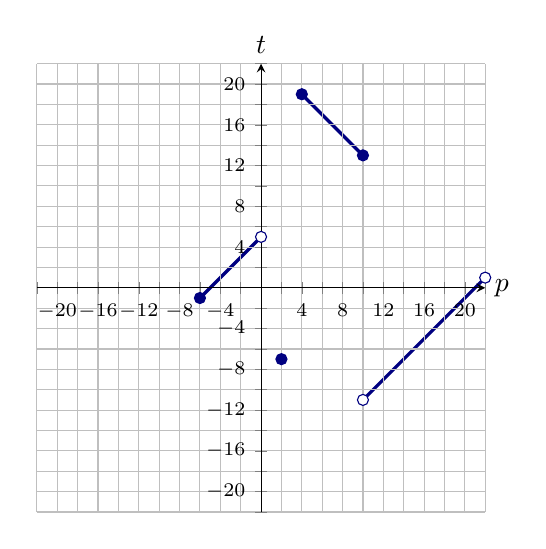
\begin{tikzpicture}
  \begin{axis}[
            domain=-22:22, ymax=22, xmax=22, ymin=-22, xmin=-22, unit vector ratio*=1 1 1,
            grid = both, 
            ytick={-22,-20,-18,-16,-14,-12,-10,-8,-6,-4,-2,2,4,6,8,10,12,14,16,18,20,22}, xtick={-22,-20,-18,-16,-14,-12,-10,-8,-6,-4,-2,2,4,6,8,10,12,14,16,18,20,22},
            yticklabels={ ,$-20$, ,$-16$, ,$-12$, ,$-8$, ,$-4$, , ,$4$, ,$8$, ,$12$, ,$16$, ,$20$, }, xticklabels={ ,$-20$, ,$-16$, ,$-12$, ,$-8$, ,$-4$, , ,$4$, ,$8$, ,$12$, ,$16$, ,$20$, },
            ticklabel style={font=\scriptsize},
            axis lines =center, xlabel=$p$, ylabel=$t$,
            every axis y label/.style={at=(current axis.above origin),anchor=south},
            every axis x label/.style={at=(current axis.right of origin),anchor=west},
            axis on top
          ]
          
        \addplot [draw=penColor,very thick,smooth,domain=(-6:0)] {x+5};
        \addplot [draw=penColor,very thick,smooth,domain=(4:10)] {-x+23};
        \addplot [draw=penColor,very thick,smooth,domain=(10:22)] {x-21};


        \addplot[color=penColor,only marks,mark=*] coordinates{(-6,-1)}; 
        \addplot[color=penColor,fill=white,only marks,mark=*] coordinates{(0,5)}; 

        \addplot[color=penColor,only marks,mark=*] coordinates{(2,-7)}; 

        \addplot[color=penColor,only marks,mark=*] coordinates{(4,19)}; 
        \addplot[color=penColor,only marks,mark=*] coordinates{(10,13)}; 
        \addplot[color=penColor,fill=white,only marks,mark=*] coordinates{(10,-11)}; 
        \addplot[color=penColor,fill=white,only marks,mark=*] coordinates{(22,1)}; 


    \end{axis}
\end{tikzpicture}
\end{image}






\textbf{What Happened?} \\

Our new function was defined by 

\[
T(p) = -2G\left( \frac{1}{2} p - 4 \right) + 1
\]






On the inside of the domain parentheses, we have $\frac{1}{2} p - 4$.  Remember, $h$ is the variable representing domain numbers of $G$. The new function has $h = \frac{1}{2} p - 4$. Solving for $p$, gives us $p = 2(h+4)$.  Now we can read off the arithmetic according to the \textbf{order of operations}.  




When looking at $p = 2(h+4)$, the parentheses are grouping symbols here.  We perform the arithmetic inside these parentheses first. \\

First, add $4$. The graph should shift to the \wordChoice{\choice[correct]{right} \choice{left}} $4$. \\
Second, multiplication by $2$. The graph should stretch horizontally by a factor of $2$.




On the outside of $G(h)$, we have multiplication by $-2$ and then addition of $1$.  These are applied in the order of operations. \\

First, multiplication by $-2$. This is negative, so the graph should flip vertically over the horizontal axis. 

\begin{itemize}
\item All positive second coordinates become negative.
\item All negative second coordinates become positive.
\item All $\answer{0}$ second coordinates remain $\answer{0}$.
\end{itemize}





The graph should also stretch vertically by a factor of $2$.  Adding $1$ shifts the whole graph \wordChoice{\choice[correct]{up} \choice{down}} $1$.








\end{example}




Take another look at the functions from the example above.









\begin{image}
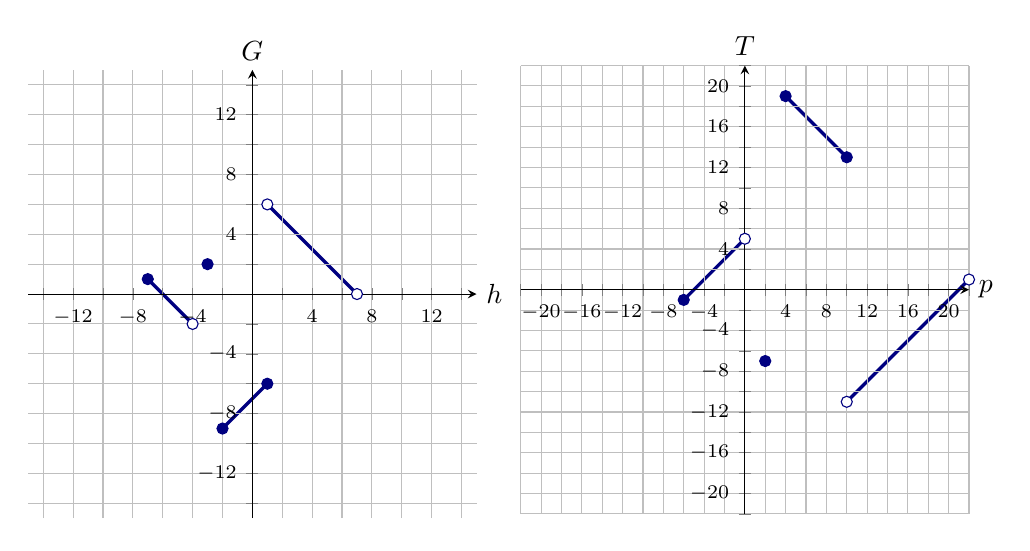
\begin{tikzpicture}
  \begin{axis}[name = leftgraph,
            domain=-15:15, ymax=15, xmax=15, ymin=-15, xmin=-15, unit vector ratio*=1 1 1,
            grid = both, 
            ytick={-14,-12,-10,-8,-6,-4,-2,2,4,6,8,10,12,14}, 
            xtick={-14,-12,-10,-8,-6,-4,-2,2,4,6,8,10,12,14},
            yticklabels={ , $-12$, , $-8$, ,$-4$, , ,$4$, ,$8$, ,$12$}, 
            xticklabels={ , $-12$, , $-8$, ,$-4$, , ,$4$, ,$8$, ,$12$},
            ticklabel style={font=\scriptsize},
            axis lines =center, xlabel=$h$, ylabel=$G$,
            every axis y label/.style={at=(current axis.above origin),anchor=south},
            every axis x label/.style={at=(current axis.right of origin),anchor=west},
            axis on top
          ]
          
        \addplot [draw=penColor,very thick,smooth,domain=(-7:-4)] {-x-6};
        \addplot [draw=penColor,very thick,smooth,domain=(-2:1)] {x-7};
        \addplot [draw=penColor,very thick,smooth,domain=(1:7)] {-x+7};

        \addplot[color=penColor,only marks,mark=*] coordinates{(-3,2)}; 
  
        \addplot[color=penColor,only marks,mark=*] coordinates{(-7,1)}; 
        \addplot[color=penColor,fill=white,only marks,mark=*] coordinates{(-4,-2)}; 
        \addplot[color=penColor,only marks,mark=*] coordinates{(-2,-9)}; 
        \addplot[color=penColor,only marks,mark=*] coordinates{(1,-6)}; 
        \addplot[color=penColor,fill=white,only marks,mark=*] coordinates{(1,6)}; 
        \addplot[color=penColor,fill=white,only marks,mark=*] coordinates{(7,0)}; 



    \end{axis}
  \begin{axis}[at={(leftgraph.outer east)},anchor=outer west,
            domain=-22:22, ymax=22, xmax=22, ymin=-22, xmin=-22, unit vector ratio*=1 1 1,
            grid = both, 
            ytick={-22,-20,-18,-16,-14,-12,-10,-8,-6,-4,-2,2,4,6,8,10,12,14,16,18,20,22}, 
            xtick={-22,-20,-18,-16,-14,-12,-10,-8,-6,-4,-2,2,4,6,8,10,12,14,16,18,20,22},
            yticklabels={ ,$-20$, ,$-16$, ,$-12$, ,$-8$, ,$-4$, , ,$4$, ,$8$, ,$12$, ,$16$, ,$20$, }, 
            xticklabels={ ,$-20$, ,$-16$, ,$-12$, ,$-8$, ,$-4$, , ,$4$, ,$8$, ,$12$, ,$16$, ,$20$, },
            ticklabel style={font=\scriptsize},
            axis lines =center, xlabel=$p$, ylabel=$T$,
            every axis y label/.style={at=(current axis.above origin),anchor=south},
            every axis x label/.style={at=(current axis.right of origin),anchor=west},
            axis on top
          ]
          
        \addplot [draw=penColor,very thick,smooth,domain=(-6:0)] {x+5};
        \addplot [draw=penColor,very thick,smooth,domain=(4:10)] {-x+23};
        \addplot [draw=penColor,very thick,smooth,domain=(10:22)] {x-21};


        \addplot[color=penColor,only marks,mark=*] coordinates{(-6,-1)}; 
        \addplot[color=penColor,fill=white,only marks,mark=*] coordinates{(0,5)}; 

        \addplot[color=penColor,only marks,mark=*] coordinates{(2,-7)}; 

        \addplot[color=penColor,only marks,mark=*] coordinates{(4,19)}; 
        \addplot[color=penColor,only marks,mark=*] coordinates{(10,13)}; 
        \addplot[color=penColor,fill=white,only marks,mark=*] coordinates{(10,-11)}; 
        \addplot[color=penColor,fill=white,only marks,mark=*] coordinates{(22,1)}; 


    \end{axis}



\end{tikzpicture}
\end{image}




\begin{enumerate}
\item On both graphs there are three line segments and one isolated point.
\item On both graphs the longest line segment has two hollow endpoints
\item On both graphs there is a short line segment with solid and one hollow endpoint. 
\item On both graphs the line segments in (a) and (c) are parallel.
\item On both graphs there is a third line segment, which is perpendicular to the other two and it has solid endpoints.
\end{enumerate}




The transformations did not change the relative shape of the graph.



All of the relative graphical relationships within each graph is also a relationship in the other graph. \\

















\begin{example}  Transformation

Let $B(r) = \frac{1}{2}|3r-1| + 4$. \\

$B$ appears to be a linear transformation of the basic absolute value function: $|x|$.

\textbf{Thinking Ahead}


The basic absolute value function has a formula like $|x|$, with $\mathbb{R}$ as its domain. The graph has a corner at $(0,0$) and a ``V'' shape.  This shape can't change from a linear transformation.

The graph of $B$ is also a ``V'', with a corner. The corner occurs where $\answer{3r-1}=0$, which is when $r=\frac{1}{3}$.  The corner is at $\left( \frac{1}{3}, \answer{4} \right)$

The outside coefficient of the transformation is $\frac{1}{2}$, which is positive.  Therefore the ``V'' will again open up for the graph of $B$.

The ``V'' is made of two rays emanating from the corner.  Therefore, we just need another point on each ray to plot the graph.

We can randomly choose any numbers on either side of $\frac{1}{3}$, like $r=-5$ and $r=5$.

$B(-5) = 12$ and $B(5) = 11$, giving us the points $\left(\answer{-5}, \answer{12}\right)$ and $\left(\answer{5}, \answer{11}\right)$, respectively.

We can now draw the graph of $y = B(r)$.









\begin{image}
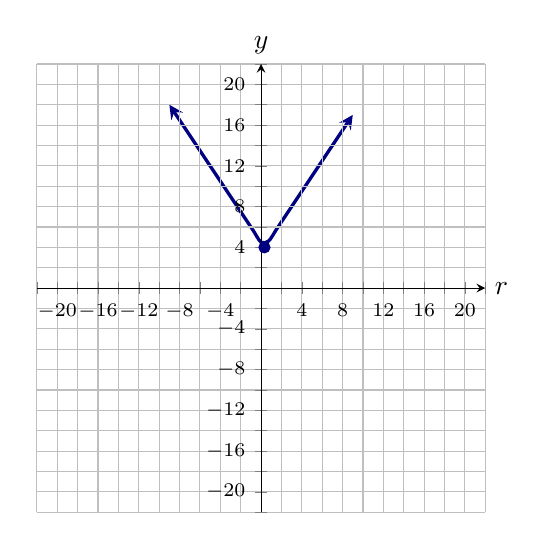
\begin{tikzpicture}
  \begin{axis}[
            domain=-22:22, ymax=22, xmax=22, ymin=-22, xmin=-22, unit vector ratio*=1 1 1,
            grid = both, 
            ytick={-22,-20,-18,-16,-14,-12,-10,-8,-6,-4,-2,2,4,6,8,10,12,14,16,18,20,22}, 
            xtick={-22,-20,-18,-16,-14,-12,-10,-8,-6,-4,-2,2,4,6,8,10,12,14,16,18,20,22},
            yticklabels={ ,$-20$, ,$-16$, ,$-12$, ,$-8$, ,$-4$, , ,$4$, ,$8$, ,$12$, ,$16$, ,$20$, }, 
            xticklabels={ ,$-20$, ,$-16$, ,$-12$, ,$-8$, ,$-4$, , ,$4$, ,$8$, ,$12$, ,$16$, ,$20$, },
            ticklabel style={font=\scriptsize},
            axis lines =center, xlabel=$r$, ylabel=$y$,
            every axis y label/.style={at=(current axis.above origin),anchor=south},
            every axis x label/.style={at=(current axis.right of origin),anchor=west},
            axis on top
          ]
          
        \addplot [draw=penColor,very thick,smooth,domain=(-9:9),<->] {0.5*abs(3*x-1)+4};

        \addplot[color=penColor,only marks,mark=*] coordinates{(0.333,4)}; 



    \end{axis}
\end{tikzpicture}
\end{image}





What are the graphical affects?


$\blacktriangleright$ Horizontally

The original inside was just $x$.  This became $3r-1$ in the new function.   

$x = 3r - 1$

But let's rephrase this to show the arithmetic performed on the original variable, $x$.

$\frac{1}{3} (x + 1)$

The order of operations tell is to add $1$ first.  That shifts the graph to the right by $1$.  Then multiplication by $\frac{1}{3}$ compresses the graph horizontally.

The orginal corner was at $x=0$.  This moved right to $1$ and then was compressed to $\frac{1}{3}$.



$\blacktriangleright$ Vertically

The original vertical measurements are given by the whole function: $|x|$.  On the outside, we multiplied by $\frac{1}{2}$, which compressed the graph vertically.  Then we added $4$, which sifted the graph vertically by $4$.

The original corner was at a height of $0$.  This was compressed to $0$ and then raised to $4$.

The new corner is at $\left( \frac{1}{3}, 4 \right)$






\end{example}

































\begin{example}  Transformation

Here is a graph of $y=k(A)$











\begin{image}
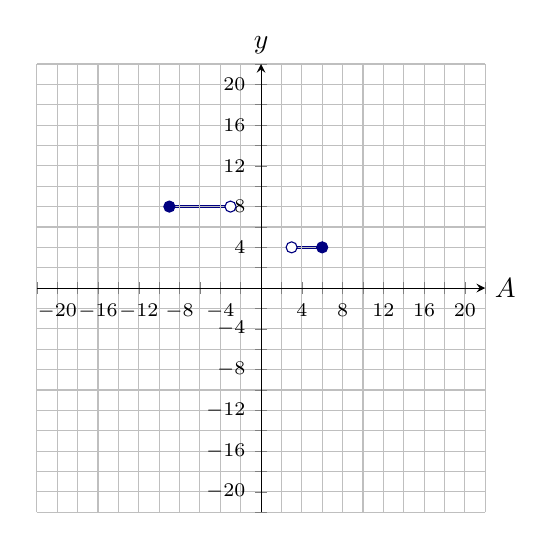
\begin{tikzpicture}
  \begin{axis}[
            domain=-22:22, ymax=22, xmax=22, ymin=-22, xmin=-22, unit vector ratio*=1 1 1,
            grid = both, 
            ytick={-22,-20,-18,-16,-14,-12,-10,-8,-6,-4,-2,2,4,6,8,10,12,14,16,18,20,22}, xtick={-22,-20,-18,-16,-14,-12,-10,-8,-6,-4,-2,2,4,6,8,10,12,14,16,18,20,22},
            yticklabels={ ,$-20$, ,$-16$, ,$-12$, ,$-8$, ,$-4$, , ,$4$, ,$8$, ,$12$, ,$16$, ,$20$, }, xticklabels={ ,$-20$, ,$-16$, ,$-12$, ,$-8$, ,$-4$, , ,$4$, ,$8$, ,$12$, ,$16$, ,$20$, },
            ticklabel style={font=\scriptsize},
            axis lines =center, xlabel=$A$, ylabel=$y$,
            every axis y label/.style={at=(current axis.above origin),anchor=south},
            every axis x label/.style={at=(current axis.right of origin),anchor=west},
            axis on top
          ]
          
        \addplot [draw=penColor,very thick,smooth,domain=(-9:-3)] {8};
        \addplot [draw=penColor,very thick,smooth,domain=(3:6)] {4};

        \addplot[color=penColor,only marks,mark=*] coordinates{(-9,8)}; 
        \addplot[color=penColor,fill=white,only marks,mark=*] coordinates{(-3,8)}; 
        \addplot[color=penColor,fill=white,only marks,mark=*] coordinates{(3,4)}; 
        \addplot[color=penColor,only marks,mark=*] coordinates{(6,4)}; 



    \end{axis}
\end{tikzpicture}
\end{image}

The graph of $k(A)$ has a shape with important or strategic points.

\begin{itemize}

\item The domain of $k$ is the union of two intervals: $[-9,-3) \cup (3,6]$.  

\item The longer interval is twice as long as the shorter interval. 

\item The inner endpoints are hollow on the graph.

\item The outer endpoints are solid on the graph.


\end{itemize}

A linear transformation will maintain this shape. \\





$\blacktriangleright$  Define $f(m)$ by 


\[
f(m) = -2 \, k\left(-\frac{1}{2} m + 1\right) - 5
\]



What will the graph of $z = f(m) = -2 k\left(-\frac{1}{2} m + 1\right) - 5$ look like? \\



$A = -\frac{1}{2} m + 1$  gives us $m = \answer{-2(A-1)}$. 

Reading the order of operations, for $-2(A-1)$, the graph will shift \wordChoice{\choice[correct]{left} \choice{right}} $\answer{1}$. Then, the graph will reflect about the vertical axis, then the graph will stretch horizontally by a factor of $\answer{2}$.



The order of operations can be read directly on the outside.  Reflect vertically, then stretch by a factor of $2$, then shift down $\answer{5}$.

$k$ only had two values, $8$ and $4$. For $f(m)$, these values will become $-2 \cdot 8 - 5 = \answer{-21}$ and $-2 \cdot 4 - 5 = \answer{-13}$.  

The horizontal endpoints of the intervals will become


\begin{itemize}
\item $-2(-9-1) = \answer{20}$
\item $-2(-3-1) = \answer{8}$
\item $-2 \left( \answer{3}-1 \right) = -4$
\item $-2 \left(\answer{6}-1 \right) = -10$
\end{itemize}






The graph of $z = f(m)$.




\begin{image}
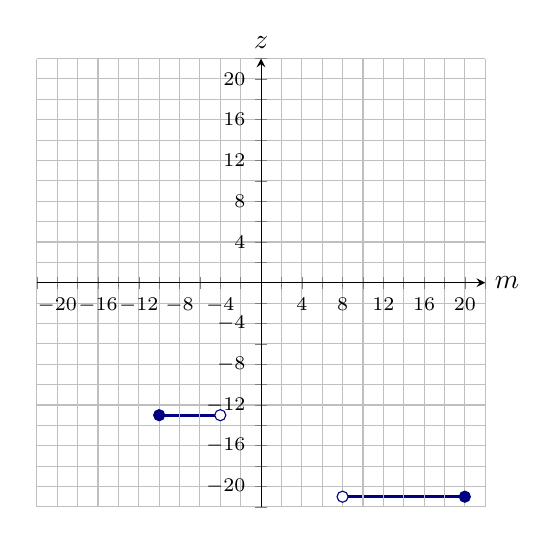
\begin{tikzpicture}
  \begin{axis}[
            domain=-22:22, ymax=22, xmax=22, ymin=-22, xmin=-22, unit vector ratio*=1 1 1,
            grid = both, 
            ytick={-22,-20,-18,-16,-14,-12,-10,-8,-6,-4,-2,2,4,6,8,10,12,14,16,18,20,22}, xtick={-22,-20,-18,-16,-14,-12,-10,-8,-6,-4,-2,2,4,6,8,10,12,14,16,18,20,22},
            yticklabels={ ,$-20$, ,$-16$, ,$-12$, ,$-8$, ,$-4$, , ,$4$, ,$8$, ,$12$, ,$16$, ,$20$, }, xticklabels={ ,$-20$, ,$-16$, ,$-12$, ,$-8$, ,$-4$, , ,$4$, ,$8$, ,$12$, ,$16$, ,$20$, },
            ticklabel style={font=\scriptsize},
            axis lines =center, xlabel=$m$, ylabel=$z$,
            every axis y label/.style={at=(current axis.above origin),anchor=south},
            every axis x label/.style={at=(current axis.right of origin),anchor=west},
            axis on top
          ]
          
        \addplot [draw=penColor,very thick,smooth,domain=(8:20)] {-21};
        \addplot [draw=penColor,very thick,smooth,domain=(-10:-4)] {-13};

        \addplot[color=penColor,only marks,mark=*] coordinates{(20,-21)}; 
        \addplot[color=penColor,fill=white,only marks,mark=*] coordinates{(8,-21)}; 
        \addplot[color=penColor,fill=white,only marks,mark=*] coordinates{(-4,-13)}; 
        \addplot[color=penColor,only marks,mark=*] coordinates{(-10,-13)}; 



    \end{axis}
\end{tikzpicture}
\end{image}



The length of the longer interval is $\answer{12}$.  The length of the shorter interval is $\answer{6}$.  Twice as long. \\

The inner endpoints are \wordChoice{\choice[correct]{hollow} \choice{solid}} on the graph. \\

The outer endpoints are \wordChoice{\choice{hollow} \choice[correct]{solid}} on the graph. \\



The longer interval is now on the right, because multiplication by $-\frac{1}{2}$ reflected the graph \wordChoice{\choice[correct]{horizontally} \choice{vertically}}. \\


The longer interval is now on the bottom, because multiplication by $-2$ reflected the graph \wordChoice{\choice{horizontally} \choice[correct]{vertically}}. \\


\end{example}


The shape didn't change.  The relative relationships were maintained within each graph.



























\subsection*{Just the Algebra}











The equation relating two functions tells us the algebraic transformations for the domain and range. \\

We just need to read it correctly. \\



\textbf{\textcolor{blue!55!black}{$\blacktriangleright$}}  Suppose we have a function $H$ with the set $[-5, 1) \cup (7, 11]$ as its domain and the set $(-3, 9]$ as its range. \\

Let's use $d$ to represent domain values of $H$.  That means $d$ represents the numbers $[-5, 1) \cup (7, 11]$. \\

Then, the symbol $H(d)$ represents the numbers $(-3, 9]$, \\


\textbf{\textcolor{blue!55!black}{$\blacktriangleright$}} Now let's introduce a second function called $P$, which is related to $H$. \\

Let's choose $k$ to represent the domain values of $P$. \\


\textbf{\textcolor{blue!55!black}{$\blacktriangleright$}} Let's suppose that $P$ and $H$ are related by the equation 

\[ 
P(k) = 4 H(k-1) - 2
\]



\textbf{\textcolor{blue!55!black}{What can we say about $P$?}}  \\



\subsection*{Domain}


We would like to collect information about the domain of $P$. \\

We know that $P(k) = 4 H(k-1) - 2$.

$k$ is representing the domain values of $P$.  If we can figure out what values $k$ can have, then we would know what values are in the domain of $P$. \\

So, what do we know about $k$? \\


We know that $k-1$ represents domain values of $H$.  We know this because the equation uses the notation $H(k-1)$.  The expression inside the parentheses represents the domain values of $H$.  That's what function notation means. \\


That means $k-1$ represents the values  $[-5, 1) \cup (7, 11]$.


\[
k - 1 \in [-5, 1) \cup (7, 11]
\]


\[
k \in [-4, 2) \cup (8, 12]
\]



We now know the values that $k$ can represent, which means we know the domain of $P$. \\












\subsection*{Range}


We would like to collect information about the range of $P$. \\

In other words, we would like to know the function values of $P$. \\ 


We know that $P(k) = 4 H(k-1) - 2$.\\


Or, we know that $P = 4 H - 2$. \\



We know that $H$ represents the values $(-3, 9]$. \\


Then, $4 H$ represents the values $(4 \cdot -3, 4 \cdot 9] = (-12, 36]$ \\



Then, $4 H - 2$ represents the values $(-12 - 2, 36 - 2] = (-14, 34]$ \\


But $P = 4 H - 2$.  Therefore, $P$ represents the values $(-14, 34]$. \\


The range of $P$ is $(-14, 34]$.






\begin{example}




\textbf{\textcolor{blue!55!black}{$\blacktriangleright$}}  Suppose we have a function $m$ with the set $[-7, 11)$ as its domain and the set $(-12, 8]$ as its range. \\

Let's use $y$ to represent domain values of $m$.  



\begin{question}

That means $y$ represents the numbers 

\[
\left[ \answer{-7}, \answer{11} \right)
\]

\end{question}





\begin{question}

Then, the symbol $m(y)$ represents the numbers

\[
\left( \answer{-12}, \answer{8} \right]
\]

\end{question}




\textbf{\textcolor{blue!55!black}{$\blacktriangleright$}} Now let's introduce a second function called $W$, which is related to $m$. \\

Let's choose $t$ to represent the domain values of $W$. \\


\textbf{\textcolor{blue!55!black}{$\blacktriangleright$}} Let's suppose that $W$ and $m$ are related by the equation 

\[ 
W(t) = -2 m(3t + 2) - 5
\]





\begin{question}

In this function equation, what is representing the domain values of $W$?

\begin{multipleChoice}
\choice [correct]{$t$}
\choice {$k$}
\choice {$3k+2$}
\choice {$3t+2$}
\end{multipleChoice}

\end{question}




\begin{question}

In this function equation, what is representing the domain values of $m$?

\begin{multipleChoice}
\choice {$t$}
\choice {$k$}
\choice {$3k+2$}
\choice [correct]{$3t+2$}
\end{multipleChoice}



The expression $3t + 2$ represents what numbers?


\[
\left[ \answer{-7}, \answer{11} \right)
\]


What numbers does $t$ represent?


\[
\left[ \answer{-3}, \answer{3} \right)
\]


\end{question}



\begin{question}

What is the domain of $W$?



\[
\left[ \answer{-3}, \answer{3} \right)
\]
\end{question}



\end{example}

























\begin{example}




\textbf{\textcolor{blue!55!black}{$\blacktriangleright$}}  Suppose we have a function $m$ with the set $[-7, 11)$ as its domain and the set $(-12, 8]$ as its range. \\

Let's use $y$ to represent domain values of $m$.  



\begin{question}

That means $m$ represents the numbers 

\[
\left( \answer{-12}, \answer{8} \right]
\]

\end{question}






\textbf{\textcolor{blue!55!black}{$\blacktriangleright$}} Now let's introduce a second function called $W$, which is related to $m$. \\

Let's choose $t$ to represent the domain values of $W$. \\


\textbf{\textcolor{blue!55!black}{$\blacktriangleright$}} Let's suppose that $W$ and $m$ are related by the equation 

\[ 
W(t) = -2 m(3t + 2) - 5
\]





\begin{question}

$-2 (-12) - 5 = \answer{19}$ \\

$-2 (8) - 5 = \answer{-21}$ \\

\end{question}






\begin{question}

What are the function values of $W$?


\[
\left[ \answer{-21}, \answer{19} \right)
\]


\end{question}


\end{example}






































\begin{center}
\textbf{\textcolor{green!50!black}{ooooo-=-=-=-ooOoo-=-=-=-ooooo}} \\

more examples can be found by following this link\\ \link[More Examples of Stretching]{https://ximera.osu.edu/csccmathematics/precalculus/precalculus/transformations/examples/exampleList}

\end{center}



\end{document}
